% Chapter 1

\chapter{Introduction} % Main chapter title

\label{Chapter1} % For referencing the chapter elsewhere, use \ref{Chapter1} 

%----------------------------------------------------------------------------------------

First of all it is important to understand at least generically what is the AEgIS experiment at the CERN and which are its goals. The acronym AEgIS stands for "Antimatter Experiment: gravity, Interferometry, Spectroscopy", this research aims to verify the weak equivalence principle for antimatter. In the first part of this chapter some particulars are explained about this experiment, in the second part gAn Web is introduced in details, the main topic of this document, the application that allows the physicists to easily perform data analysis in the AEgIS experiment environment, through a web interface. 

\section{The AEgIS experiment}


\begin{figure}[H]
\centering
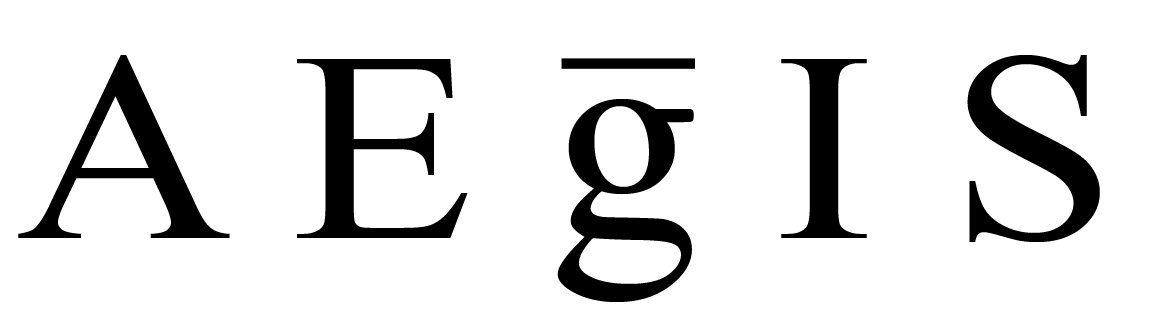
\includegraphics[scale=0.25]{aegisLogo.png} 
\caption{AEgIS's Logo}
\end{figure}

The weak equivalence principle, also known as universality of free fall, states that in the same field all bodies fall with the same acceleration, regardless of the mass and the composition. This principle has been thoroughly tested for the matter, but not for the antimatter: the most important goal of AEgIS experiment is to measure the weak equivalence principle for the antimatter; to test the universality of free fall, AEgIS will attempt to measure the gravitational interaction between matter (the Earth) and antimatter (antihydrogen). Antihydrogen is the antimatter counterpart of hydrogen, it is the simplest atom built with antimatter (see below for a description of its components). The first antihydrogen in an electromagnetic trap has been produced by the ATHENA experiment in 2012 (\url{http://www.nature.com/nature/journal/v419/n6906/full/419439a.html}) [1]
with the contribution of a group of the University of Brescia.

The AEgIS experiment is the result of a wide and international scientific collaboration, as visible in the figure 1.2.

\begin{figure}[H]
\centering 

\includegraphics[scale=0.5]{aegis_collaboration_institutes.pdf} 
\caption{Aegis Collaboration institutes}
\end{figure}


In the context of neutral antimatter, the gravitational interaction is of high interest, because it can potentially reveal new forces that violate the weak equivalence principle. Thomas Phillips, from Duke University, says: "If antimatter fell down faster, it would mean the discovery of at least one new force, probably two. If it fell up, it would mean our understanding of general relativity is incorrect". In a practical point of view AEgIS tries to measure the time of flight and the vertical displacement of antihydrogen, with a moirè deflectometer: this process is quite complex, and it is easier to explain it using the following figures (1.3, 1.4 and 1.5).

\begin{figure}[H]
\centering 
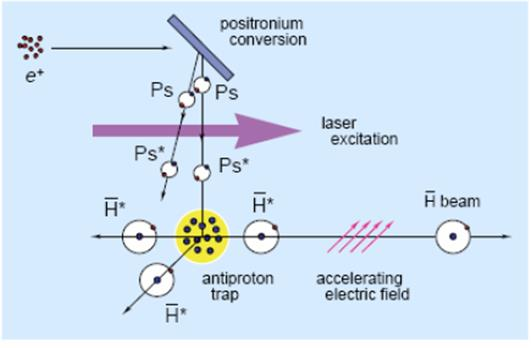
\includegraphics[scale=0.5]{AEgISScheme.png} 
\caption{AEgIS's Scheme, taken from "AEgIS experiment at CERN: measuring antihydrogen free-fall in Earth’s gravitational field to test WEP with antimatter"}
\end{figure}

In the Fig. 1.3 we can see the process that allows to create through a so called "charge-exchange" reaction antihydrogen. In few words, to create antihydrogen two ingredients are needed: antiprotons and positrons. The antiprotons are provided by CERN, while positrons are produced by the experiment with a radioactive source. To correctly explain this process we start with some definitions:


\begin{enumerate}

% 1
\item Positron: it is the counterpart of the electron in the antimatter. It is an antielectron, that is an electron with positive electrical charge. It is denoted with "e$^{+}$".

% 2
\item Positronium: it is an unstable system consisting of an electron and a positron, bound together into an exotic atom. It is denoted with $ {Ps} $.

% 3
\item Antiproton: it is the antiparticle of the proton. Antiprotons are stable, but they are typically short-lived since any collision with a proton will cause both particles to be annihilated in a neutron and to disappear creating other particles. It is indicated with $ \overline{p} $ (pronounced pbar).

% 4
\item Antihydrogen: it is the antimatter counterpart of hydrogen. Whereas the common hydrogen atom is composed of an electron and a proton, the antihydrogen atom is made up of a positron and an antiproton. It is indicated with $ \overline{H} $ (pronounced hbar).


% 5
\item Antiproton trap: a device that uses an axial magnetic field to radially confine charged particles, in this case antiprotons.


\end{enumerate}

\begin{figure}[H]
\centering
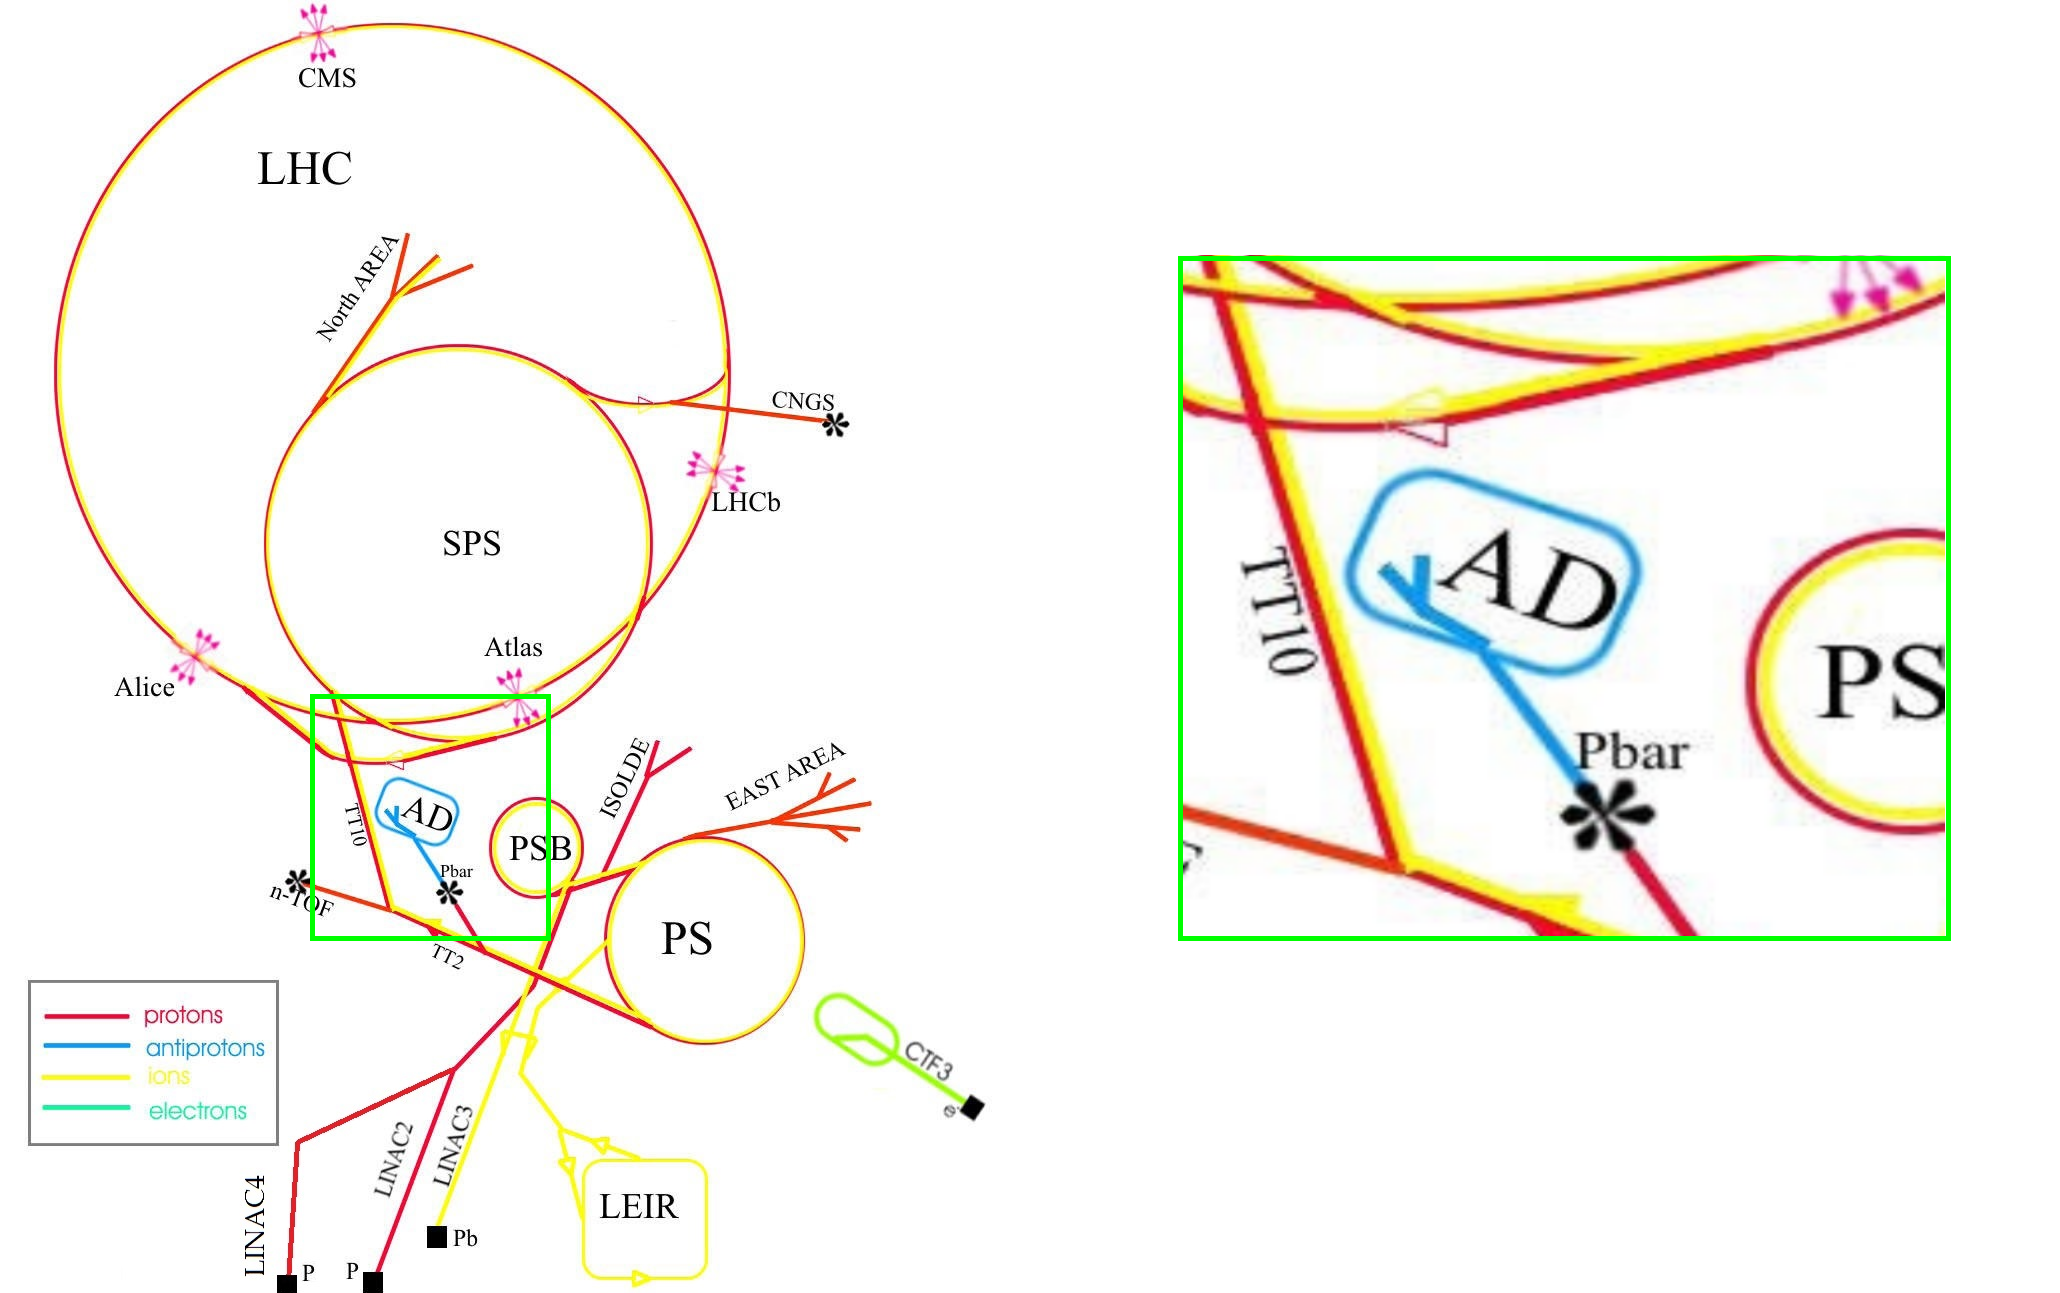
\includegraphics[scale=0.25]{CERNaccelerators.png} 
\caption{ As shown in this figure, AD in a ring in the CERN accelerator system, the AEgIS experiment is part of AD. }
\end{figure}


Antiprotons are provided by the CERN accelerator system and an electric field confines them axially. 
Protons collide with nuclei inside a metal cylinder called "target". About four proton-antiproton pairs are produced in every million collisions, and it is possible to separate antiprotons using magnetic fields. The following step is to guide antiprotons toward the AD (Antiproton Decelerator, the ring shown in figure 1.4) where they are slowed down. 
The AEgIS experiment is part of AD, that is a system able to provide a stable source of antiprotons.
To execute AEgIS experiment, antiprotons must be trapped and held inside an antiproton trap, where magnetic fields force the charged antiparticles to spiral around the magnetic field lines, and electric fields confine them along the magnetic axis.

For what concerns positrons, as represented in Fig. 1.3 a beam of positrons (that comes from a $^{22}$Na radioactive source) is accelerated and driven to collide against a "positron-positronium converter" (that is a mesoporous silica film). This process creates positronium, that needs to be excited by lasers, to reach an excited state called Rydberg State. The positronium in Rydberg state is indicated with $ {Ps*} $, it has a longer life than the unexcited positronium, and can be driven to fly into an antiproton trap.


When $ {Ps*} $ is excited by lasers it can combine itself with $ \overline{p} $ to generate excited antihydrogen ($ \overline{H}* $) and electrons. The antihydrogen beam is accelerated using an electric field towards a moiré deflectometer. Then, during the travel it decays to ground state.  


\begin{figure}[H]
\centering
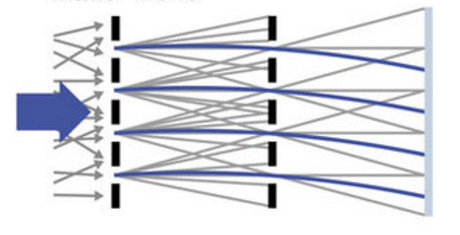
\includegraphics[scale=0.5]{MoireDeflectometer.png} 
\caption{Moiré Deflectometer's scheme, taken from \url{http://www.nature.com/articles/ncomms5538} [2]}
\end{figure}

In the Fig. 1.5 a schematic view of a moirè deflectometer is presented.
An antihydrogen beam is thrown toward two subsequent gratings that restrict the transmitted particles to well-defined trajectories. The trajectories are inflected by a force (in this case the force related to $ {m*g} $) and follow a parabolic path. In the final part of the deflectometer there is a detector that shows where the antimatter annihilates, that it is possible to compare the expected trajectories without forces with the obtained trajectories, and measure the force. The proof of principle that such system can be used with antimatter has been realized and operated with $ \overline{p} $s. It showed that a displacement of few $ \mu m $ can be detected with this technique, this result has been published in Nature [\url{https://www.nature.com/articles/ncomms5538}][2]


\begin{figure}[H]
\centering
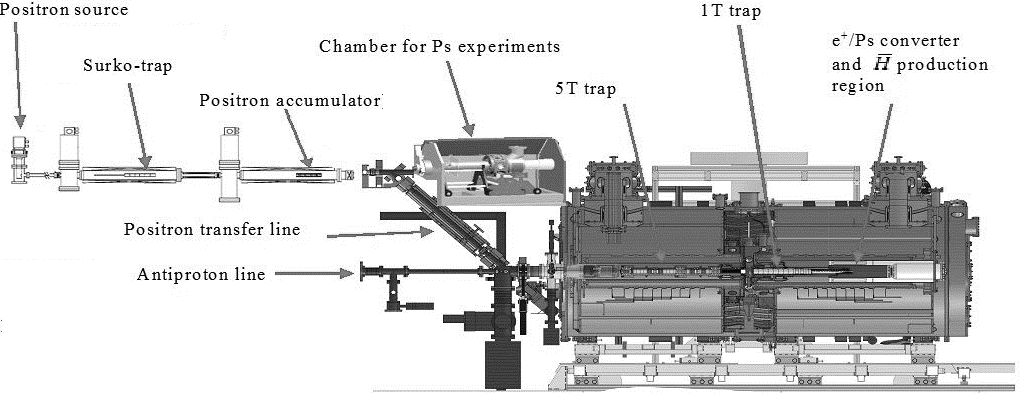
\includegraphics[scale=0.35]{SchemeMachineSetUp.png} 
\caption{AEgIS apparatus set up, taken from "AEgIS experiment at CERN: measuring antihydrogen free-fall in Earth’s gravitational field to test W.E.P. with antimatter" }
\end{figure}
